
\section{Introduction}
%Duzenleme laz?m
Computers have become increasingly more ambitious and popular, along with improvements in artificial intelligence and machine learning, to extract new information from sources such as text and video for people, or even to learn new tasks. Maintaining a safety critical hardware components must be done by step by step according to technical orders. Extracting tasks in these areas, especially sequential tasks, are sin qua none for teaching to a robot or a computer which needs to be directed by humans.  Part of speech (POS) tagging is the key topic for information retrieval for extracting the valuable information that is used for classification, clustering etc. from any natural languages. 

In this work, it is aimed to automatically model the steps of a certain task by using text data which is easily accessible from the internet and to create methods and tool that can help people. Since there are many recipe documents and videos available on the internet,  working area is selected as cooking recipes. POS tagging is significant that  it constructs a description a set of instructions of a recipes which forms content based text analysis of our work. We describe a rule-based tagger which
performs as well as taggers based upon probabilistic models. The rule-based tagger overcomes the limitations common in rule-based approaches to language processing: it is robust, and the rules are automatically acquired.


\section{Related Works}

Algorithmic processing of training texts and / or commands expressed in natural language has long been an interesting question \cite{harnad90}. In this problem, the artificial intelligence agent (such as a robot) is trying to learn the operations corresponding to symbols that are expressed in a field. The system is expected to automatically interact with definitions in the physical world as symbols to interact with objects and objects. We obtained through www.allrecipes.com.

\cite{chen2011learning} have developed a system that can act according to the expressions expressed in natural language in the system they developed. Based on the reinforced learning methods, the system can translate the sentences into natural language by using the information in the location (such as the objects on the wall) and the state flow that is modeled. As can be seen from these studies in the literature, reinforcement learning techniques are used in problems where the current situation can be modeled more clearly.

A slightly different problem is \cite{hosseini2014learning} developed a similar method for solving problems expressed in mathematical texts. According to this method, the system is mapping the problem described in the text to a set of equations and producing the result. To learn the method, we use a training set marked at different levels. Equations that can be created in the system can be given or can be learned only when the last answer is given. In the method they developed, the solution is defined as diagrams, and a probability model that maps the information given in the text to the diagram is developed. Of course, it is necessary that the structure of the questionnaire is similar and that all of them can be transferred to the equation diagram.

Recipes can also be thought of as a set of steps that must be followed. From this point of view, there are common aspects to the problems described above. The most important difference is that it is difficult to convert the media knowledge to a reward function to provide reinforcement learning. The biggest reason for this is that it is difficult to model the correct sequence of operations that can be done while cooking. To overcome this problem in the processing of recipes, three different basic approaches are striking. The first is knowledge-based methods that are dependent on previously created knowledge vocabulary, the second is those using supervised learning methods, and the third is unsupervised learning and extracting a specific model from the data in the compilation. The first approach involves all the recipes, contents, tools and processes, and methods that can show the relationship between them. In the second approach, it is necessary to generate the data with the equivalent of the text for the training compilation. In the third category, transductive learning is performed according to the solutions given, ie it is not possible to classify the given samples and to process new ones.

\subsection{Information Based Methods}

\cite{walter2011workflow} describes a method of generating flow diagrams from recipe texts, extracting recipe statements as material, processing and finishing conditions. Based on this information, a flow diagram is created. This method requires pre-tagged sentences and a dictionary that holds all of these tags.

Another problem that may be related is the creation of an information dictionary. \cite{gaillard2012interactive} foods and their relationships with a Wiki-style method. Its approach basically consists of 6 hierarchies; diet and mealtime according to different features categorize the food. With this approach it is possible to adapt a new recipe or an existing recipe.

Although food-related ontology is increasingly detailed, these methods often fail to adapt to dynamic language and variety. Thus, when ontology methods are used alone, successful results are achieved for some data sets, but success is often low. Moreover, in order to adapt these methods to a different language, ontologies should be structured in accordance with other languages.


\subsection{Supervised Learning Methods}

One of the most important features of tutorial learning techniques is the target description model. Basically, the information that this model needs to be able to show is where the processes described in the steps are done on which materials and where the output of this step is used. Some of these associations show in the tree structure \cite{jermsura}, while some researchers show it in a non-cyclic manner \cite{malmaud2014cooking}. It is possible that this notation can both express all the recipes and learn it automatically. \cite{jermsura} defined a representation in the tree data structure that stores food items and their relationships over the description steps. This demonstration can show which step of the recipes is related to which steps and materials.

\cite{malmaud2014cooking} sees text in recipes as a Markov Decision Process problem by expanding semantic role labeling. It holds two things between the process and the material. The purpose of this relationship is to demonstrate the processes within the training that cause these situations to occur.

\cite{mori2014flow} created a labeling tool by showing recipes as non-cyclic charts in their initial work. With this tool, the recipe created a graph that indicates the skis over the text. The given Japanese recipes first extract the word segmentation, locate the words in the clan's tasks, label the named entities, and finally construct the predicate-argument structure.

In order to resolve the uncertainties in the contents, \cite{greene} tagged about 180,000 sentences for labeling and edited the tags of the words in the table of contents using the Conditional Random Fields method.

\subsection{Unsupervised Learning Methods}

In 2015, \cite{kiddon2015mise} has developed a method of learning without a teacher for the processing of recipes. Unlike previous works, this method learns the linkages of the line by using different parameters according to the variables in the system and using the expectation maximization method. Since this model is constructed according to the definition in the drawing, it is not possible to learn the features of an extragalactic recipe. In this respect, it is a transduction method, all the recipes to be processed have to be obtained at the model learning time. Moreover, the generated data model has a high number of implicit variables because it defines both the verbs, the contents, and the content of the contents in relation to the steps as one of the parameters of the model. When such high numbered models are learned, they can be found in a high number of local maxima, which prevents the optimum model from being found.
It is intended to remove them as to which action is associated with the material, removing the flow of the recipe as a whole. These methods are inspired by semantic spaces used in text mining and meaning spaces that show word meaning relations. By using these material spaces, it is possible to determine which materials can be replaced instead of which materials. \cite{nedovic2013learning} used a similar method to define a method of learning materials for different types of food. Latent Dirichlet Allocation (LDA) and Deep Belief Networks (DBN) are used in the method. It has been seen that the output of the system can group materials according to the foods in different kitchens. A similar study has been proposed by \cite{achananuparp2016extracting} to produce safer food recommendations in meals. In this method, Singular Value Decomposition (SVD) method, which is widely used for extracting word meaning relations, is used.

\section{Experimental Setup}

As seen in the literature, there are many methods aiming at revealing the relationship between the description texts and the contents of the description texts, the sequence of the process flow and the situations that occur during the actions and showing them with the models by many different methods. The texts should be easily perceivable by the computer by passing about 18000 recipes we obtained through www.alrecipes.com through certain operations.

Using NLTK\cite{nltk} libraries, each of the recipes was first converted into a clean text by separating individual recipes and separating them into words, punctuation, and meaningless words.  (names, categories, contents, descriptions, and comments). Then each recipe is divided into sentences for labelling.

\begin{algorithm}
\caption{Data Retrieval and Preprocessing Overview}
\label{alg:generator}
\SetKwProg{ReadProcessData}{Function \emph{ReadProcessData}}{}{end}

\ReadProcessData{CvsFiles data}{
     \ForAll{eachRecipe $c$ in data}{
(ingredients, direction) = readDataFromCSVfile($c$)

ingreNewTag = calculateTAGWithCRF(ingredients)

tokenizedD = tokenizeSentence(direction)

taggedD = calculateTagsWithPOSTag(tokenizedD)

taggedDirection = updateTag(taggedD, ingreNewTag)
      
     }
}
\end{algorithm}

This section we prepare data for the process, firstly, read data from csv file which is generated before and divide data into two parts, direction and ingredients. Using the NLTK \cite{nltk} library, labeling was done according to the culled state (VB, NN, ADJ, etc.) that each of the belts passed. As a result of the labeling made, "I can chopped green chile peppers" in the table of contents is labeled as below in TABLE 1. It was observed that 450 of 171.224 labeled samples were separated and tested and 89 percentage correctly tagged.

\begin{table}[]
\centering
\caption{Tags}
\label{my-label}
\begin{tabular}{|l|l|l|l|l|l|}
\hline
 chop & green & chile & peppers \\ \hline
 VB      & NN    & NN    & NN      \\ \hline
\end{tabular}
\end{table}

As can be seen in Table 1, it does not allow me to know that the word "life" is a unit of measure, "1" actually tells the quantity, and that the words "green" and "choped" are actually interpretations of a "papers" word.

The challenge of parsing the recipe is to be able to distinguish content components from component cues. Erica Greene (2016) has trained 171,244 sets (labeled as UNIT, QUANTITY, COMMENT and OTHER) with the very specific set of CRF ++\cite{crf} (Conditional Random Fields) method she has created to solve this problem and has been able to label the contents portion probabilistically with a newly given description. Let us have the sentence "1 teaspoon sugar". The model is using 171,224 tagged data to learn a model that can predict the tag sequence for any sentence we have given to it, even though we have never seen this component count before. It approaches this by modeling the conditional probability of a set of labels.

p (UNIT UNIT UNIT| "1 teaspoon sugar")

p (QUANTITY UNIT UNIT| "1 teaspoon sugar")

p (UNIT QUANTITY UNIT| "1 teaspoon sugar")

p (UNIT UNIT QUANTITY "1 teaspoon sugar")

p (UNIT QUANTITY QUANTITY "1 teaspoon sugar")

p (QUANTITY QUANTITY QUANTITY | "1 teaspoon sugar")

p (UNIT QUANTITY NAME| "1 teaspoon sugar")

Secondly, tag direction and ingredients wtih the help of NLTK \cite{nltk} and CRF++\cite{crf} libraries. Tagging direction according to NLTK \cite{nltk} libraries is not satisfied in order to generate  action graph. For this reason, update and change tags after NLTK \cite{nltk} process is finished. 

\begin{algorithm}
\caption{Pos Tagging Overview}
\label{alg:generator}
\SetKwProg{updateTags}{Function \emph{updateTags}}{}{end}

\updateTags{Direction taggedDirection}{
     \ForAll{sentence in taggedDirection}{
     
   updateVerbs(sentence)
   
   updateTools(sentence)
  
   updateIngredients(sentence)   
     }
    findRelatedVerbsPair(direction) 
    }
\end{algorithm}
As mentioned above, it calculates all the probabilities that can be labeled "1 teaspoon sugar". The beauty of the linear-chain CRF model makes some conditional independence assumptions that allow us to use dynamic programming to efficiently search the area of all possible label sequences. As a result, we have re-tagged our data with Erica Greene (2016), and the result is shown in TABLE 2. The results are shown in Table 2, which shows the best label sequence at a time that is linear with the number of second.


\begin{table}[]
\centering
\caption{Tags}
\label{my-label}
\begin{tabular}{|l|l|l|l|l|l|}
\hline
chop & green & chile & peppers \\ \hline
VB     & CMMT    & NAME    & NAME      \\ \hline
\end{tabular}
\end{table}

 After, tags are updated according to neighbor tags, if the tag is "VB" and the neighbor tag is "DET" (determiners), two words are concatenated by the algorithm and tagged by "PRED" . The CRF++ algorithm is tagged each word separately but  the same tag,    these are concatenated. That is depicted on the TABLE 3 and TABLE 4. 
 
 \begin{table}[]
\centering
\caption{Tags}
\label{my-label}
\begin{tabular}{|l|l|l|l|l|l|}
\hline
put    & the     &  peppers  & into  & the    & pan \\ \hline
VB    & DET   & NAME     & ADP & DET & TOOLS      \\ \hline
\end{tabular}
\end{table}

 \begin{table}[]
\centering
\caption{Tags}
\label{my-label}
\begin{tabular}{|l|l|l|l|l|l|}
\hline
put       &  the peppers       & into  the pan \\ \hline
PRED  & INGEDIENTS & NON IGRE SPAN  \\ \hline
\end{tabular}
\end{table}

Finding action pairs with proximity values are required for graph generation. Generally, actions are sequential in the recipes, however, actions can be done  parallel or some actions take duration while doing. So that, "preheat- PRED" is related with "bake for- PRED". This results show the relation between "preheat- PRED" and "bake for- PRED". In order to link "preheat- PRED"  and  "bake for- PRED" in the graph,  we look at the similarity of the cosine with the actions. 

Sometimes, sentences might not have any actions because of the POS Tagger's errors. During POS Tagging process, if a sentence in the direction does not have an PRED tag, we try to find most probable action in the sentence with the help of bigram collocations ,which are expressions of multiple words which commonly co-occurs, in NLTK library. This process is inevitable for generating action graph. Because each sentence must have at least one action according to our algorithm. 


\subsection{Calculation of Proximity}
Kiddon et.\cite{kiddon2015mise} , some words are not in the table of contents, but more than one is meant. (Eg mixture, them) Kiddon et.\cite{kiddon2015mise} defines this as a hidden object. He has created a probabilistic model to make hidden objects clear. In order to reveal these hidden objects, we present a relationship between the words 'NAME' in this action and its contents. In fact, each word is represented as a vector and we calculate the cosine similarity between them.

Using the Word2Vec \cite{word2vec} library that displays 3.5 billion words created by a working group led by Tomas Mikolov (Google) as a 300-dimensional vector vocabulary, the words that pass through the intellectual part and are labeled 'NAME' have been converted into a 300-dimensional vector. 

In the recipe sentence set, phrases without any word labeled 'NAME' are removed. When the words labeled as 'PRED' are extracted, all the words are converted into 300 dimensional vectors and the averages are taken. Because the other words around the word tagged by "VB" can also provide us with information about what materials the hidden object contains. If you only go through the actions, you will be made a comment by looking at the similarity of only two calves. However, the sentence can sometimes contain words that characterize the words in the contents. Let's take a look at "Cook the mixture until caramelized". It is labeled as "cook-PRED". When we look at the similarity of the cosine with the contents, it is seen that almost all of them resemble to each other. However, when the complex average of sentence is taken, "caramelized" word is included. And the result is more similar to "Onion" and "sugar". Taking the average of the blame for this reason actually brings us closer to the right conclusion. 

Generating Graph is based on actions of each sentence. Action node is the main node of a sentence. If a sentence does not have a ingredient tags, the action may not be related with the next action or may not relevant  the ingredients which is used before action. In order to generate graph, we find the relations between the actions which do not related with the ingredients.
Using Word2Vec, we calculate the cosine similarity between the action which does not have any relations with ingredients and whole actions in the direction.

Firstly, each action node is generated and linked with related nodes of ingredients and nodes of tools, when the action node generation is finished, linking actions process begins. Actions are generally sequential in the direction. However, some actions are related with specific action or relevant with the next action in the direction. "preheat" is the action which is related with "bake for" action. Because after  the "preheat the oven" action , "bake for the mixture" can be done. This "preheat" action should be before the "bake for" action. "preheat" action  result is related with "bake for" action. In order to find this relation and similarity about whole actions in the direction, we use Word2Vec library for finding cosine similarity between the actions. If the similarity bigger that threshold value that we select, the pairs and the similarity value are held  in the list. Then the list is used for linking the action nodes in the graph. This process is expressed in the following algorithm Graph Generation and Validation. 



\begin{algorithm}
\caption{Graph Generation and Validation}
\label{alg:generateGraph}
\SetKwProg{generateGraph}{Function \emph{generateGraph}}{}{end}
\generateGraph{taggedRecipe recipe, verbPairs, pairs}{
actionNodeList =[]

     \ForAll{sentence  in recipe}{
     	actionN = generateSentNode(sentence)
	actionNodeList.append(actionN)
    
     }
     
     \ForAll{action in actionNodeList}{
    	linkTheAction(action, pairs)
     }
}
\end{algorithm}
        

\section{Results}

33 hand labelled recipes, which is used byKiddon et. al \cite{kiddon2015mise},  are used  in the algorithm. POS Tagging results are more promising than Kiddon et. al \cite{kiddon2015mise} that is depicted Table 7. When we look at an example on a "hot chicken salat" recipe, full text is in the Table 5, finding actions in Imperative sentences are really problematic to tag. For this reason we add "I WOULD" prefix to sentences before tagging. 



    
\begin{table}[]
\centering
\caption{Hot Chicken Salad}
\label{my-label}
\begin{tabular}{|l|l|}
\hline
\textbf{No} & \textbf{Direction}                                                                                                                                 \\ \hline
1           & Preheat oven to 350 degrees F (175 degrees C).                                                                                                     \\ \hline
2           & \begin{tabular}[c]{@{}l@{}}Combine the chicken, celery, almonds,\\ bell pepper, onion, pimento, salt, \\ lemon juice, and mayonnaise.\end{tabular} \\ \hline
3           & Mix well and pour into a 1 1/2 quart casserole dish.                                                                                               \\ \hline
4           & Top with grated cheese and the crushed potato chips.                                                                                               \\ \hline
5           & Bake for 25 minutes or until cheese is melted.                                                                                                     \\ \hline
\end{tabular}
\end{table}

After standard tagging in NLTK\cite{nltk}, we rename tags which we define, and concatenate words which are related to each others that is shown on the Table 6. Ingredients tagging with the help of CRF++ \cite{crf} is satisfiable especially when we compare to hand labelled data. 

 Supervised learning methods as CRF++ \cite{crf} is implemented our method for extracting ingredients since we are using previously tagged data from NYTimes \cite{greene}, The result of correctly tagged data is shown in the Table 7.  The results are promising than the other works because of supervised learning. We describe a rule-based tagger which
performs as well as taggers based upon probabilistic models. The rule-based tagger overcomes the limitations common in rule-based approaches especially using supervised learning in language processing: it is upstanding, and the results is 88.64  as regards with F1 measurement. 

As a result the, action graph of the given recipes described in Table 5 is depicted on Figure 1.  

\begin{table}[]
\centering
\caption{Tagged Sentence Example}
\label{my-label}
\begin{tabular}{|l|l|}
\hline
\textbf{Our Tagged Data}                                                                                                                                                                                                                                                                                                                                                                                                                                                  & \textbf{Hand Labelled Data}                                                                                                                                                                                                                                                                                                                                                                                                                                                     \\ \hline
\begin{tabular}[c]{@{}l@{}}SENT : combine the chicken ,\\  celery , almonds , bell pepper,\\  onion , pimento , salt , \\ lemon juice , and mayonnaise .\\ PRED : combine\\ INGREDIENTS : chicken\\ INGREDIENTS : celery\\ INGREDIENTS : almonds\\ INGREDIENTS : bell pepper\\ INGREDIENTS : onion\\ INGREDIENTS : pimento\\ INGREDIENTS : salt\\ INGREDIENTS : lemon juice\\ INGREDIENTS : mayonnaise\\ DOBJ : the chicken\end{tabular} & \begin{tabular}[c]{@{}l@{}}SENT: combine the chicken , \\ celery , almonds , bell pepper , \\ onion , pimento , salt ,\\ lemon juice , and mayonnaise.\\ PRED: combine\\ INGREDIENTS: chopped salted \\ almonds\\ INGREDIENTS: salt\\ INGREDIENTS: chopped green \\ bell pepper,\\ INGREDIENTS: mayonnaise,\\ INGREDIENTS: chopped celery,\\ INGREDIENTS: minced onion,\\ INGREDIENTS: lemon juice,\\ INGREDIENTS: chopped pimento\\  peppers\\ DOBJ : the chicken\end{tabular} \\ \hline
\end{tabular}
\end{table}


\begin{figure*}
  \centering 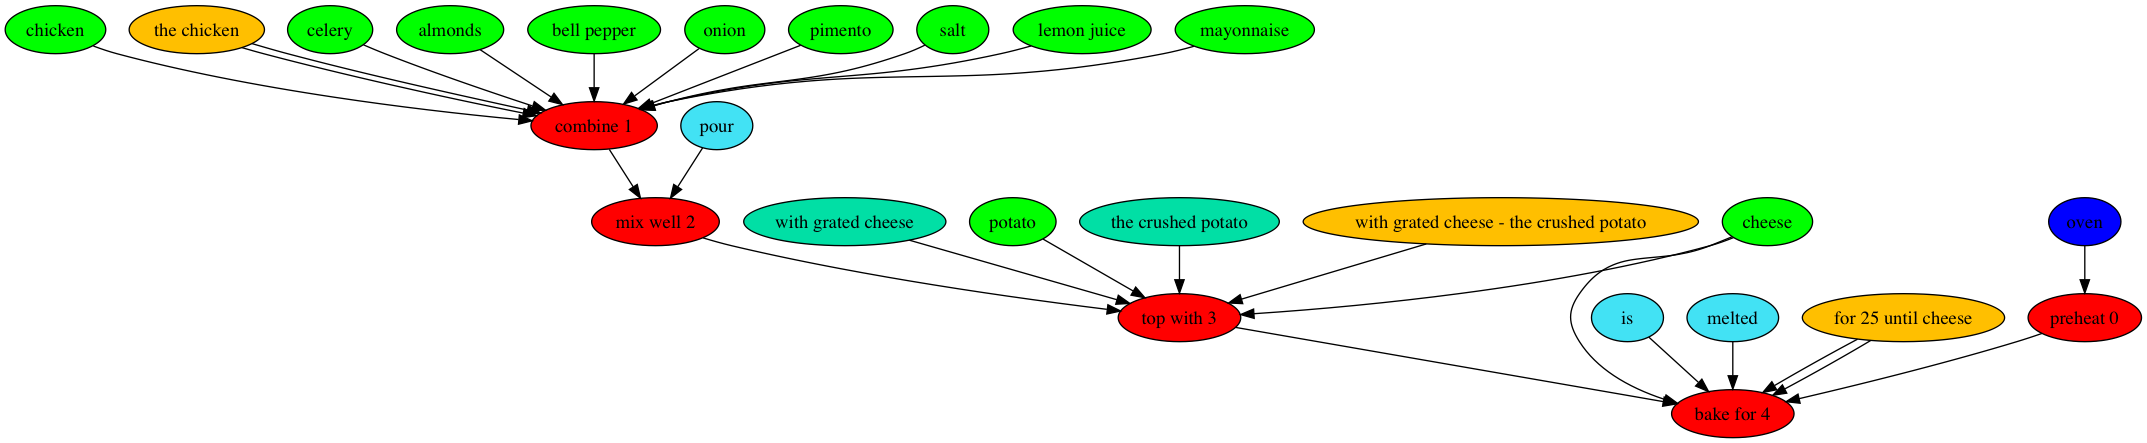
\includegraphics[width=\textwidth]{hot-chicken-salad.png}
  \caption{Hot-Chicken Salad Action Graph}
\end{figure*}


 \begin{table}[]
\centering
\caption{Experiment Results}
\label{my-label}
\begin{tabular}{|l|l|l|l|l|l|}
\hline
 .    & \textbf{Precision}     &  \textbf{Recall}  & \textbf{F1} \\ \hline
\textbf{Our work}    &  88.64    & 76.47 & 82.10      \\ \hline
Kiddon et. al \cite{kiddon2015mise}   & 68.7& 65.0 & 66.8 \\ \hline
\end{tabular}
\end{table}


\section{Conclusions}
We presented semi-supervised methods for segmenting to tag actions and ingredients in recipe text. Our model uses CRF models to identify tags and uses Word2Vec \cite{word2vec} model to keep the ordering of actions to achieve a complete graph. This graph  can convert to a computer readable format that any automation software  use it easily. 

Our model outperformed a strong linear baseline, while learning a variety of domain knowledge, such as verb signatures and probable ingredient components for different composites. Future work includes learning a more comprehensive model of locations (e.g., identify- ing nested locations such as an oven and a pan in the oven), enriching action graphs with greater se- mantic coverage (e.g., durations, tools, amounts), and training and evaluating on larger datasets. We also plan to use our techniques to support related tasks, such as instructional recipe generation.


%\end{document}  % This is where a 'short' article might terminate

%\appendix

%\begin{acks}
  %TODO
%\end{acks}
